% Interpreting sASM via information propagation + over-counting (1D/2D Laplace).
% Minimal academic style, English.  Compile: pdflatex (x2).  Figures from infoprop.c.
\documentclass[aspectratio=169,10pt]{beamer}
\usepackage[T1]{fontenc}
\usepackage{lmodern}
\usepackage{amsmath,amssymb,bm}
\usepackage{booktabs}
\usepackage{graphicx}
\graphicspath{{../../asm_bug_demo/infoprop_out/}}

\definecolor{Struct}{HTML}{1F3A5F}
\definecolor{Gray}{HTML}{6E6E6E}
\definecolor{Accent}{HTML}{8C2D04}
\usetheme{default}
\usefonttheme{professionalfonts}
\setbeamertemplate{navigation symbols}{}
\setbeamercolor{structure}{fg=Struct}
\setbeamercolor{frametitle}{fg=Struct}
\setbeamerfont{frametitle}{series=\bfseries,size=\large}
\setbeamercolor{block title}{fg=white,bg=Struct}
\setbeamercolor{block body}{bg=Struct!6}
\setbeamercolor{block title alerted}{fg=white,bg=Accent}
\setbeamercolor{block body alerted}{bg=Accent!8}
\setbeamertemplate{frametitle}{\vskip0.45em\hspace{0.2em}\usebeamerfont{frametitle}\insertframetitle%
  {\ifx\insertframesubtitle\empty\else\\[0.1em]\small\color{Gray}\insertframesubtitle\fi}\par}
\setbeamertemplate{footline}{\hfill\footnotesize\color{Gray}\insertframenumber\,/\,\inserttotalframenumber\hspace{0.4cm}\vspace{3pt}}
\renewcommand{\arraystretch}{1.2}
\newcommand{\Nc}{N_{\mathrm c}}

\begin{document}

% ===== Title =====
\begin{frame}[plain]
  \vskip1.0cm
  {\color{Struct}\large\bfseries Why does sASM work --- and only when the subdomain solve is inexact?\par}
  \vskip0.5em
  {\color{Gray} An interpretation through information propagation and overlap over-counting\par}
  \vskip0.9em\hrule height0.4pt\vskip0.7em
  \footnotesize
  Minimal 1D / 2D Laplace experiment (all numerics in PETSc): BASIC vs.\ sASM additive Schwarz,\\[0.2em]
  with \emph{exact} (Cholesky) and \emph{inexact} (ICC(0)) subdomain solves.\\[0.3em]
  1D: 256 DOF, 8 subdomains.\qquad 2D: $64^2$ grid, $4\times4$ subdomains.
\end{frame}

% ===== The result that frames everything =====
\begin{frame}{The result that frames everything}
\framesubtitle{CG iterations to $\|r\|/\|b\|<10^{-8}$, same problem, only the subdomain solver changes}
\begin{center}
\begin{tabular}{l cc cc}
\toprule
 & \multicolumn{2}{c}{\textbf{1D} Laplace} & \multicolumn{2}{c}{\textbf{2D} Laplace} \\
\cmidrule(lr){2-3}\cmidrule(lr){4-5}
 & exact & ICC(0) & exact & ICC(0) \\
\midrule
BASIC & 15 & 15 & 23 & \textbf{102} \\
sASM  & 25 & 25 & 27 & \textbf{67} \\
\bottomrule
\end{tabular}
\end{center}
\vskip0.5em
\begin{itemize}\itemsep0.35em
  \item \textbf{sASM beats BASIC only in one cell: 2D with an inexact solve} (67 vs 102).
        Everywhere else sASM $\approx$ or slightly worse than BASIC.
  \item 1D ``ICC'' $=$ exact: a tridiagonal matrix has no fill, so ICC(0) is the complete Cholesky.
        Hence 1D cannot show the anomaly at all.
  \item \textbf{Question:} what makes the \emph{inexact} solve bad, and why does sASM fix it precisely there?
\end{itemize}
\end{frame}

% ===== Fig 1: over-counting =====
\begin{frame}{Mechanism, part 1: BASIC over-counts the overlap}
\framesubtitle{one preconditioner apply $\sum_i R_i^{\top}A_i^{-1}R_i\,r$ to a localized residual}
\begin{center}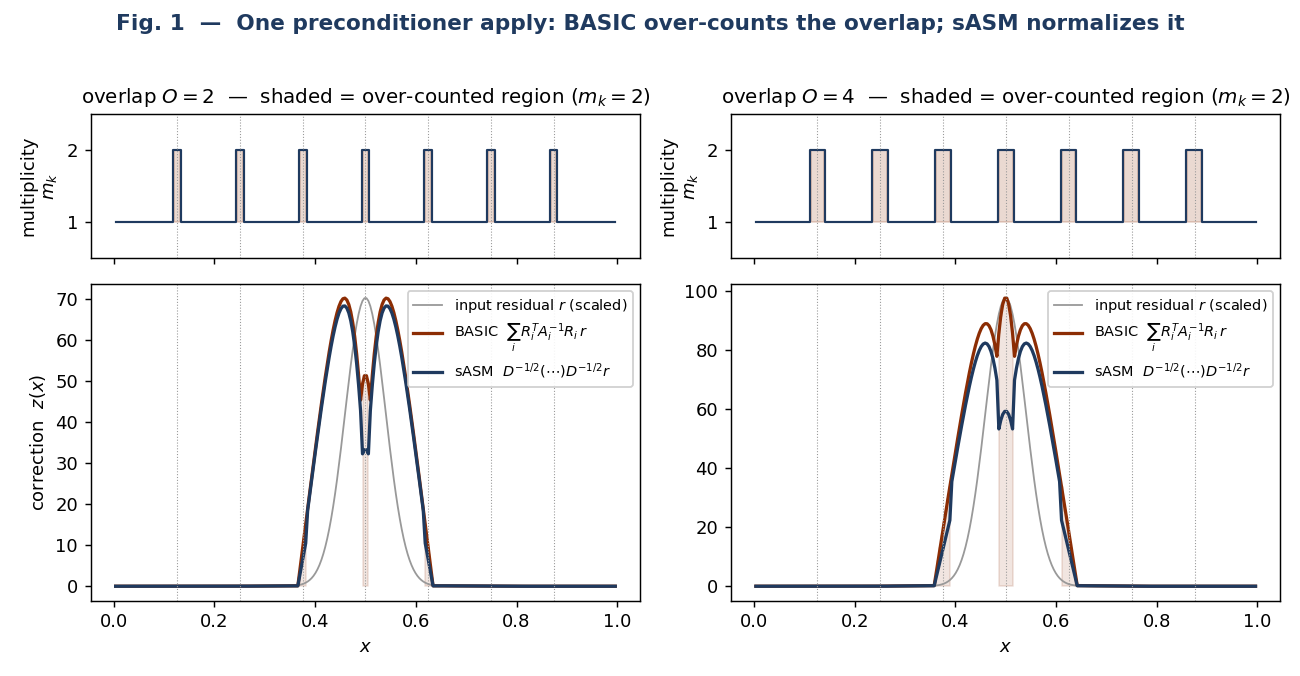
\includegraphics[width=0.92\textwidth]{fig1_overcount}\end{center}
\vskip-0.2em
\begin{itemize}\itemsep0.2em\footnotesize
  \item In the overlap a DOF belongs to $m_k$ subdomains, so its correction is \emph{added} $m_k$ times.
  \item \textbf{BASIC} (red) bumps up at every overlap seam; \textbf{sASM} (blue) is normalized by $1/\sqrt{m_k}$.
  \item This over-count is the algebraic fact $\sum_i R_i^{\top}R_i=\mathbf D=\mathrm{diag}(m_k)$. It is harmless \emph{by itself} --- the next slides show when it bites.
\end{itemize}
\end{frame}

% ===== Fig 2: information propagation =====
\begin{frame}{Mechanism, part 2: information propagates one subdomain per iteration}
\begin{columns}[T]
\begin{column}{0.6\textwidth}
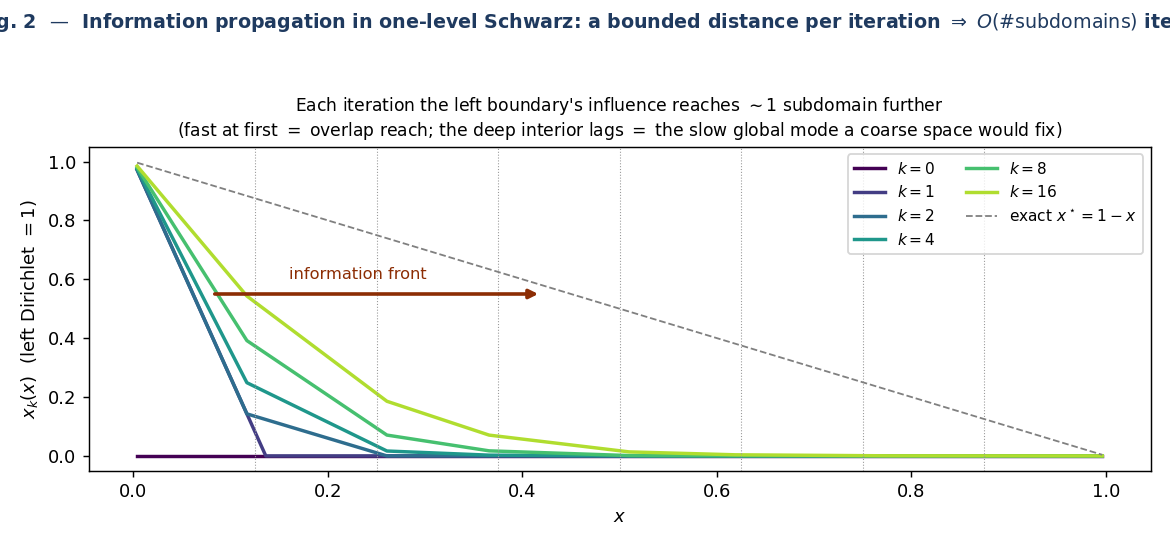
\includegraphics[width=\textwidth]{fig2_front}
\end{column}
\begin{column}{0.4\textwidth}
\footnotesize
\begin{itemize}\itemsep0.3em
  \item Laplace is globally coupled, but each Schwarz step solves only \emph{local} problems.
  \item So the boundary's influence advances $\sim$1 subdomain per iteration (fast at first $=$ overlap reach).
  \item The deep interior lags --- that slow global mode is what a coarse space (two-level) would remove.
  \item \textbf{One-level cost is $O(\#\text{subdomains})$ iterations}, independent of BASIC vs sASM.
        Overlap helps by speeding this propagation.
\end{itemize}
\end{column}
\end{columns}
\end{frame}

% ===== Q1: why inexact is bad =====
\begin{frame}{Q1 --- Why is the inexact (ICC) solve bad?}
\framesubtitle{the abstract Schwarz bound: the two factors \emph{multiply}}
\[
\kappa(\mathbf M^{-1}\mathbf A)\ \le\ C_0^2\ \cdot\
\underbrace{\omega}_{\substack{\text{(A) inexactness}\\ \text{exact}=1,\ \text{ICC}>1}}\ \cdot\
\underbrace{\Nc}_{\substack{\text{(B) over-count}\\ \text{(colouring / }m_k)}}
\]
\begin{itemize}\itemsep0.28em
  \item \textbf{Exact} ($\omega{=}1$): each local correction is the \emph{exact} local solution; over-counting only lifts $\lambda_{\max}\!\le\!\Nc$ --- bounded, CG tolerates it. \emph{No anomaly} (table: 23 vs 27).
  \item \textbf{ICC} ($\omega{>}1$): each local correction carries an \emph{error}, and BASIC \textbf{adds $m_k$ of these errors} in the overlap. They do not cancel --- they accumulate:
  \begin{itemize}\footnotesize\itemsep0.15em
    \item $\lambda_{\max}\le \omega\,\Nc$: the inexactness is \emph{multiplied} by the over-count;
    \item wider overlap makes the block bigger, so fixed-fill ICC is a worse approximation ($\omega\!\uparrow$) \emph{and} $\Nc\!\uparrow$ --- so $\kappa$ \emph{rises} with overlap (the anomaly).
  \end{itemize}
  \item The accumulated, amplified error \textbf{piles up at the subdomain seams} and the outer CG must clear it.
\end{itemize}
\end{frame}

% ===== Q1 evidence: Fig 3 + Fig 4 =====
\begin{frame}{Q1 --- the evidence}
\begin{columns}[T]
\begin{column}{0.52\textwidth}
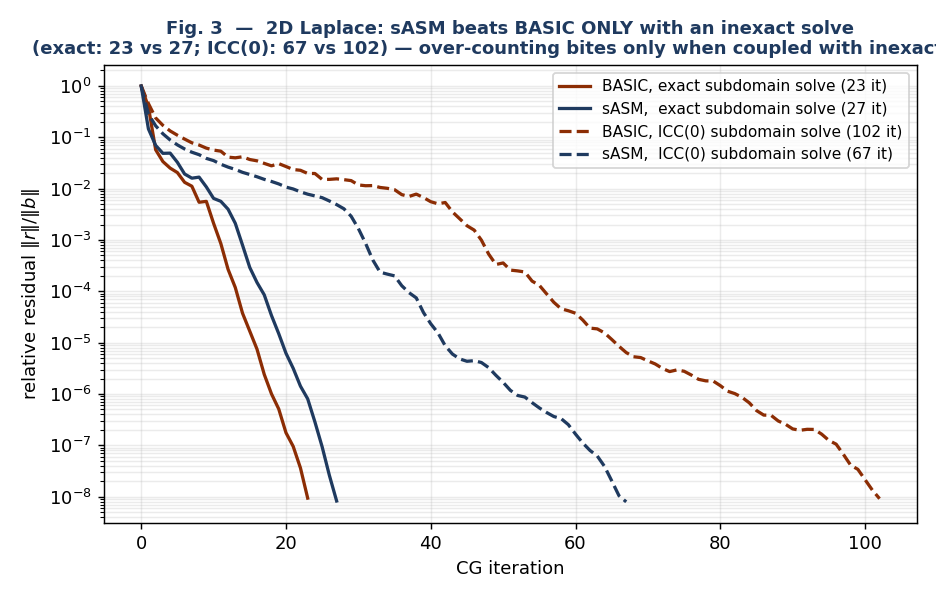
\includegraphics[width=\textwidth]{fig3_reshist2d}
\vskip-0.1em
{\footnotesize \textbf{Residual history.} Exact: BASIC$\approx$sASM (both fast). ICC: BASIC \textbf{102} blows up.}
\end{column}
\begin{column}{0.48\textwidth}
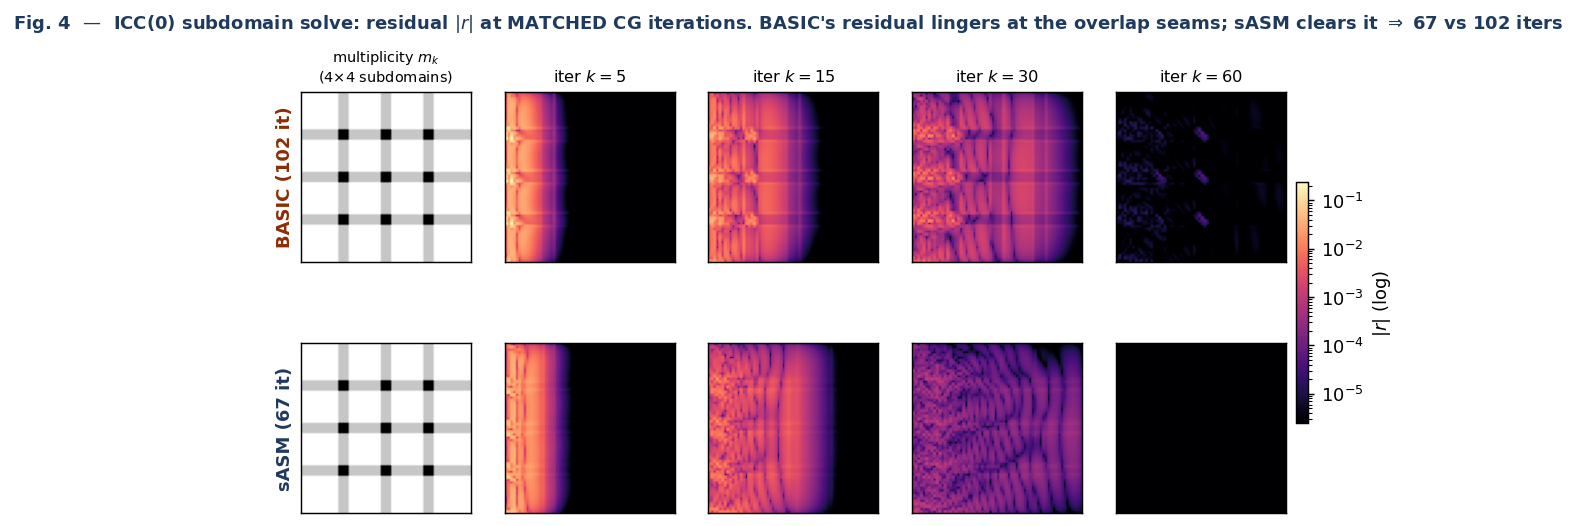
\includegraphics[width=\textwidth]{fig4_heatmap2d}
\vskip-0.1em
{\footnotesize \textbf{ICC residual field} at matched CG iterations: at $k{=}60$ BASIC is still bright (error not cleared), the seams lit up by the over-counted ICC error.}
\end{column}
\end{columns}
\vskip0.35em
\centering
\begin{beamercolorbox}[wd=0.92\textwidth,sep=4pt,rounded=true]{block body alerted}
\footnotesize ``Inexact is bad'' $=$ the local error is \textbf{counted $m_k$ times in the overlap} (A$\times$B), accumulating into seam residual that costs iterations --- and worsens as overlap grows.
\end{beamercolorbox}
\end{frame}

% ===== Fig 5: overlap sweep =====
\begin{frame}{Q1, deeper --- the seam error grows with overlap}
\framesubtitle{2D Laplace, $128^2$, $8\times8$ subdomains, ICC(0); residual $|r|$ at fixed iteration $k{=}40$}
\begin{center}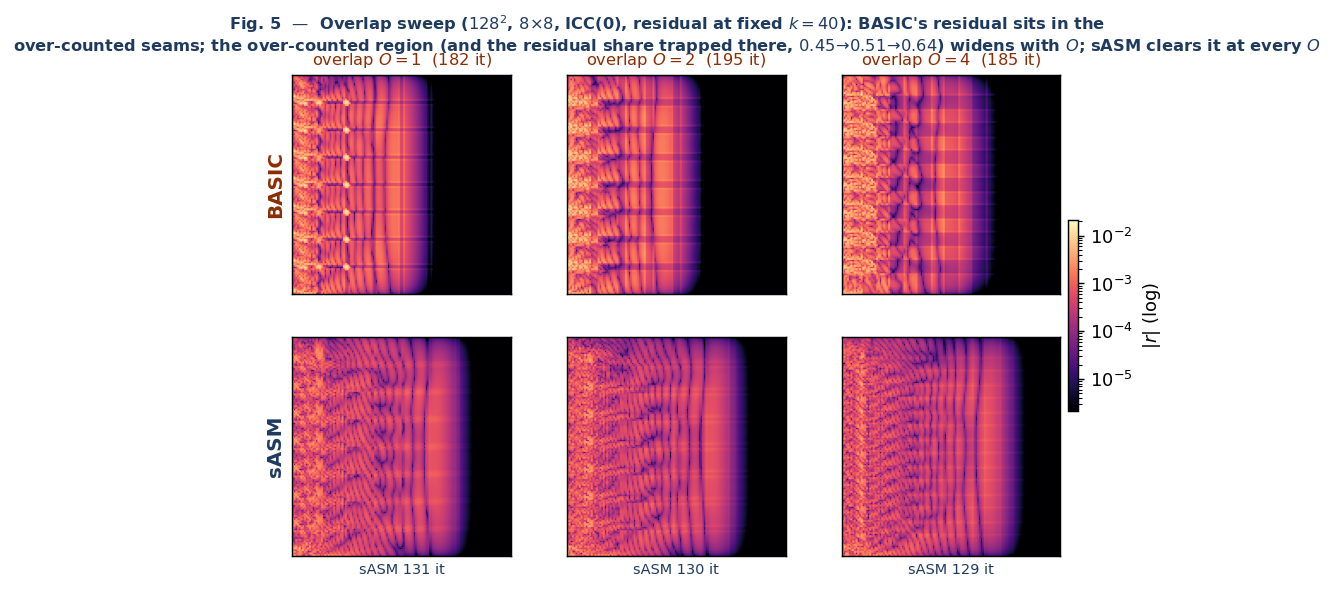
\includegraphics[width=0.86\textwidth]{fig5_overlap_sweep}\end{center}
\vskip-0.2em
\begin{itemize}\itemsep0.15em\footnotesize
  \item The over-counted seam region \emph{widens} with overlap, and the residual share trapped there grows $0.45\!\to\!0.51\!\to\!0.64$.
  \item sASM is better at \emph{every} overlap (iters BASIC 182/195/185 vs sASM 131/130/129).
  \item Honest note: in 2D the iteration count vs $O$ is non-monotone (ICC is only mildly inexact in 2D). The clean monotone ``overlap$\uparrow\Rightarrow$iter$\uparrow$'' is a 3D effect $\to$ next slide.
\end{itemize}
\end{frame}

% ===== Fig 6: 3D real Sys3 =====
\begin{frame}{The same effect on the real 3D problem (Sys 3)}
\framesubtitle{mixed Dirichlet/Neumann Laplace, $n_x{=}48$, 4 ranks --- the actual torso-type solve}
\begin{center}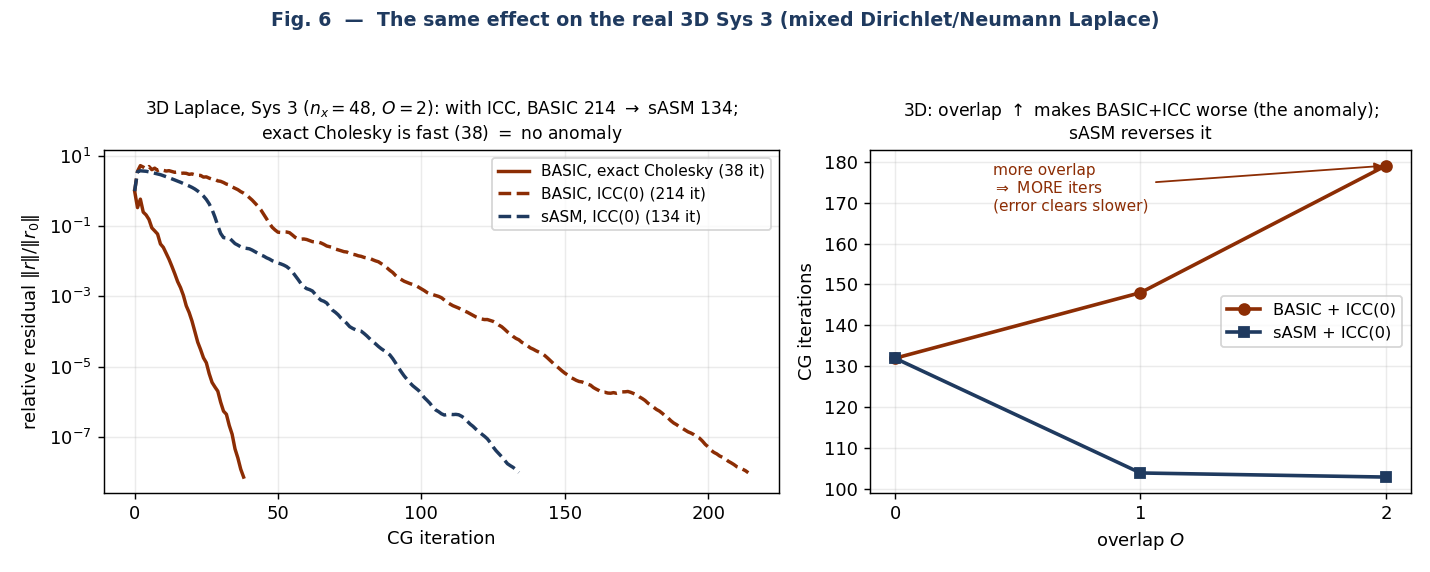
\includegraphics[width=0.95\textwidth]{fig6_3d}\end{center}
\vskip-0.2em
\begin{itemize}\itemsep0.12em\footnotesize
  \item \textbf{Left:} ICC --- BASIC 214 slow, sASM 134 recovers; exact Cholesky 38 (no anomaly, the reference).
  \item \textbf{Right:} the clean monotone anomaly --- BASIC$+$ICC $132\!\to\!148\!\to\!179$ (more overlap, more iters $=$ error clears slower); sASM $132\!\to\!104\!\to\!103$ reverses it.
\end{itemize}
\end{frame}

% ===== Q2: why sASM fixes it =====
\begin{frame}{Q2 --- Why does sASM overcome it?}
\framesubtitle{$\mathbf M_{\mathrm{sASM}}^{-1}=\mathbf D^{-1/2}\big(\textstyle\sum_i R_i^{\top}A_i^{-1}R_i\big)\mathbf D^{-1/2}$, partition of unity $\sum_i d_i^2=1$}
\[
\text{BASIC: } \lambda_{\max}\le \omega\,\Nc
\qquad\xrightarrow{\ \mathbf D^{-1/2}(\cdot)\mathbf D^{-1/2}\ }\qquad
\text{sASM: } \lambda_{\max}\le \omega
\]
\begin{itemize}\itemsep0.3em
  \item The $\mathbf D^{-1/2}$ sandwich normalizes the overlap so each DOF's correction is counted \textbf{once}: the over-count factor $\Nc$ is \textbf{removed} (Fig.~1, blue is flat).
  \item \textbf{This breaks the multiplication.} The inexactness $\omega$ is no longer multiplied by $\Nc$: the ICC error in the overlap is counted once, \emph{not accumulated} $\Rightarrow$ no seam pile-up.
  \item Result (ICC): the seam residual clears (Fig.~4, sASM nearly dark at $k{=}60$); CG recovers \textbf{102 $\to$ 67}.
  \item \textbf{sASM does not fix the inexactness} ($\omega$ is still $>1$) --- it stops the over-count from \emph{amplifying} it. So $\kappa\sim C_0^2\,\omega$, and overlap helps again.
\end{itemize}
\end{frame}

% ===== concept: what is the subdomain solve =====
\begin{frame}{What does ``exact / inexact subdomain solve'' actually solve?}
\framesubtitle{$A_i=R_iAR_i^{\top}$ --- the global Laplace restricted to subdomain $i$ (with overlap)}
\begin{itemize}\itemsep0.45em
  \item $A_i$ implicitly imposes \textbf{homogeneous Dirichlet} on the \emph{artificial cut} between subdomains (the cross-interface coupling is dropped), and keeps the physical BC on faces that touch the real boundary.
  \item \textbf{Exact solve} $A_i^{-1}$ (Cholesky) $=$ \emph{exactly} solving a local Dirichlet--Laplace subproblem. $\;\omega=1$.
  \item \textbf{Inexact solve} ICC(0) $=$ exactly solving a \emph{perturbed} operator $\tilde A_i=A_i-E_i$, where $E_i$ is the fill that ICC(0) \emph{drops}. Equivalently, the same Dirichlet subproblem solved only approximately. This $E_i$ \textbf{is} the source of $\omega>1$, and its error sits in the overlap/seam.
\end{itemize}
\vskip0.3em
\begin{block}{So ``inexact'' is not mysterious}
\footnotesize ICC(0) keeps only $A_i$'s nonzero pattern and throws away all fill-in. Whether that loses anything depends entirely on the \textbf{ordering} of the unknowns --- next slide.
\end{block}
\end{frame}

% ===== Fig 7: reordering makes ICC inexact =====
\begin{frame}{Reordering the unknowns turns the ICC inexact}
\framesubtitle{same subdomains / overlap / weights --- only the ICC \emph{ordering} changes (natural / RCM / random)}
\begin{center}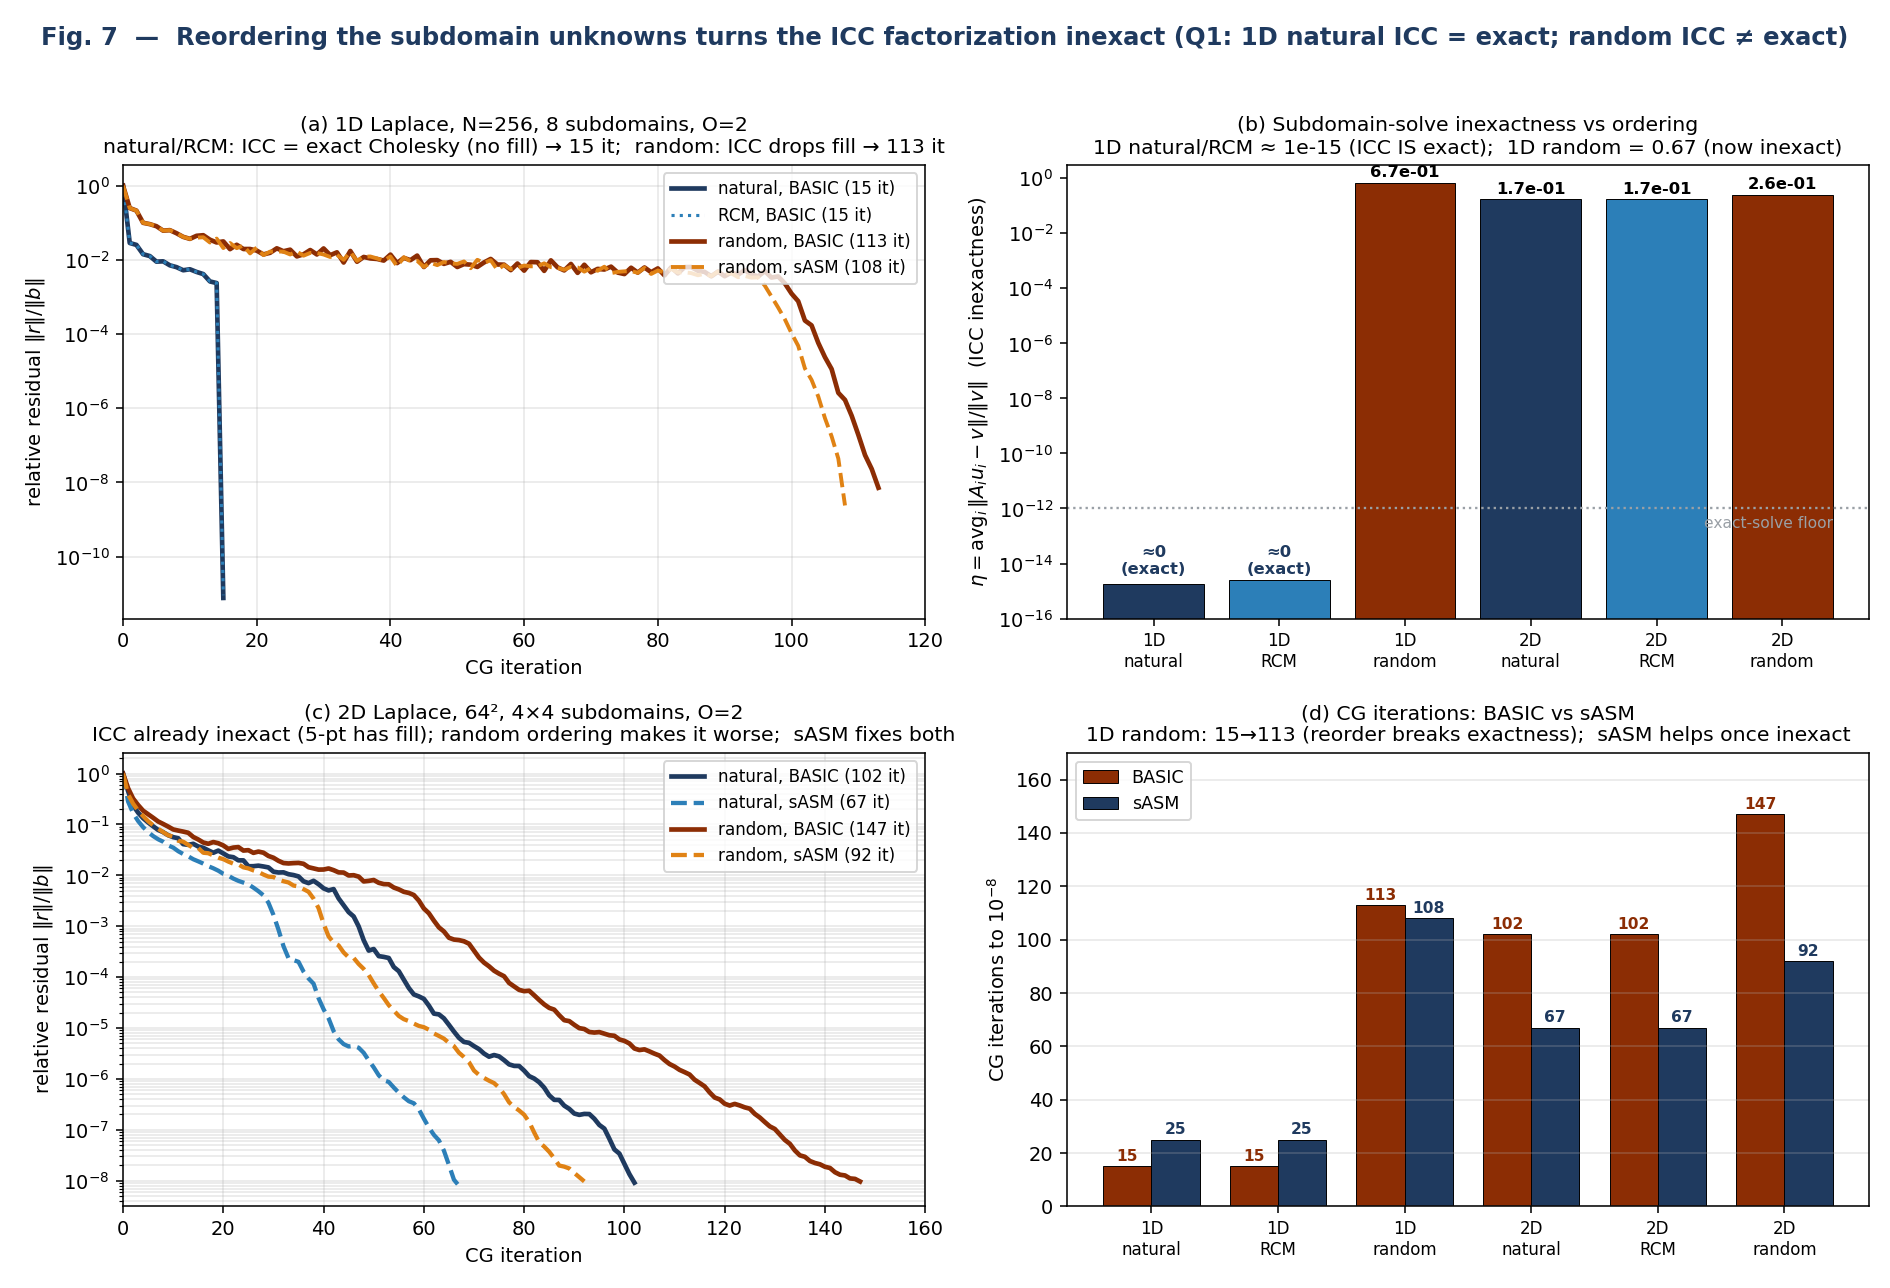
\includegraphics[width=0.97\textwidth]{fig7_reorder}\end{center}
\vskip-0.25em
\begin{itemize}\itemsep0.1em\footnotesize
  \item \textbf{(b)} the headline: 1D \emph{natural} \& \emph{RCM} give $\eta\approx10^{-15}$ --- ICC \emph{is} exact Cholesky (a tridiagonal has no fill); 1D \emph{random} gives $\eta=0.67$ --- ICC is now genuinely inexact.
  \item \textbf{(a)/(d)} 1D: natural/RCM converge in 15 it; random blows up to 113 (exactness destroyed). RCM keeps 1D banded, so it stays exact --- not every permutation breaks it, only a band-widening (random) one.
  \item \textbf{(c)/(d)} 2D: the 5-point ICC already has fill ($\eta{=}0.17$); random makes it worse ($\eta{=}0.26$), $102\!\to\!147$ it; sASM repairs both ($102\!\to\!67$, $147\!\to\!92$), more so the more inexact the solve.
\end{itemize}
\end{frame}

% ===== Conclusion =====
\begin{frame}{Conclusion}
\begin{block}{The one-sentence picture}
\footnotesize
BASIC counts the overlap twice (Fig.~1). With \emph{exact} solves that is harmless --- it only lifts
$\lambda_{\max}$, which CG tolerates (Fig.~3, solid). With an \emph{inexact} ICC solve the local error is
counted $m_k$ times, so ``inexactness $\times$ over-count'' accumulates at the seams (Fig.~4) and convergence
degrades (Fig.~3, dashed, 102). sASM's $\mathbf D^{-1/2}$ partition of unity removes the over-count, breaking
that product, so the inexact corrections are no longer amplified and CG recovers (102 $\to$ 67).
\end{block}
\vskip0.3em
\begin{itemize}\itemsep0.3em
  \item \textbf{Q1:} inexactness is bad because BASIC \emph{multiplies} it by the overlap over-count $\Nc$;
        and both grow with overlap, so iterations rise with overlap.
  \item \textbf{Q2:} sASM removes $\Nc$ (partition of unity), so the inexactness is no longer amplified --- it helps \emph{exactly} when the solve is inexact, and is neutral when it is exact.
  \item Information always propagates $\sim$1 subdomain/iteration (Fig.~2): a one-level cost, untouched by either method.
\end{itemize}
\end{frame}

\end{document}
